\documentclass[pdf]{beamer}
\newcommand{\quotes}[1]{``#1''}

\mode<presentation>
{
  \usetheme{Warsaw}
  \useoutertheme{infolines}
  \usecolortheme[RGB={28,13,151}]{structure}
  %\usetheme[height=7mm]{Rochester}
  % or ...

  \setbeamercovered{invisible}
  % or whatever (possibly just delete it)
}

\usepackage{ upgreek }
\usepackage{verbatim} 
\usepackage{listings}
\usepackage{tikz}
\usetikzlibrary{arrows}
\usetikzlibrary{shapes}
\tikzstyle{block}=[draw opacity=0.7,line width=1.4cm]

\lstloadlanguages{C++}
\lstnewenvironment{code}
	{%\lstset{	numbers=none, frame=lines, basicstyle=\small\ttfamily, }%
	 \csname lst@SetFirstLabel\endcsname}
	{\csname lst@SaveFirstLabel\endcsname}
\lstset{% general command to set parameter(s)
	language=C++, basicstyle=\footnotesize\ttfamily, keywordstyle=\slshape,
	emph=[1]{tipo,usa}, emphstyle={[1]\sffamily\bfseries},
	morekeywords={tint,forn,forsn},
	basewidth={0.47em,0.40em},
	columns=fixed, fontadjust, resetmargins, xrightmargin=5pt, xleftmargin=15pt,
	flexiblecolumns=false, tabsize=2, breaklines,	breakatwhitespace=false, extendedchars=true,
	numbers=left, numberstyle=\tiny, stepnumber=1, numbersep=9pt,
	frame=l, framesep=3pt,
}
\usepackage{multicol}

\usepackage[spanish]{babel}
% or whatever

\usepackage[utf8]{inputenc}
% or whatever

\usepackage{times}
\usepackage[T1]{fontenc}
% Or whatever. Note that the encoding and the font should match. If T1
% does not look nice, try deleting the line with the fontenc.
\usepackage{enumitem}
\usepackage{booktabs}


\title[Prueba de oposición] % (optional, use only with long paper titles)
{Prueba de oposición - Algoritmos 2016}

\author[Brian Bokser] % (optional, use only with lots of authors)
{Brian Bokser}
% - Give the names in the same order as the appear in the paper.
% - Use the \inst{?} command only if the authors have different
%   affiliation.
\institute[UBA-FCEN] % (optional, but mostly needed)
{
  Facultad de Ciencias Exactas y Naturales\\
  Universidad de Buenos Aires
}


% Ac� se puede insertar el logo de la UBA
% \pgfdeclareimage[height=0.5cm]{university-logo}{university-logo-filename}
% \logo{\pgfuseimage{university-logo}}


% Delete this, if you do not want the table of contents to pop up at
% the beginning of each subsection:
\AtBeginSubsection[]
{

  \begin{frame}<beamer>{Contenidos}
    \tableofcontents[currentsection,currentsubsection]
  \end{frame}
	
}


% If you wish to uncover everything in a step-wise fashion, uncomment
% the following command: 

%\beamerdefaultoverlayspecification{<+->}


\begin{document}
\pgfdeclarelayer{background}
\pgfsetlayers{background,main}
\begin{frame}
  \titlepage
\end{frame}

\begin{frame}{Contenidos}
  \tableofcontents
  % You might wish to add the option [pausesections]
\end{frame}



\section{Introducci\'on}

\begin{frame}{Introducción}

\newtheorem{enun}{Enunciado}


\begin{enun}
    \par{
    La cantidad de parejas en desorden de un arreglo A[1 . . . n] es la cantidad de parejas de posiciones 1 $\leq$ i <
    j $\leq$ n tales que A[i] > A[j]. Dar un algoritmo que calcule la cantidad de parejas en desorden de un arreglo
    y cuya complejidad temporal sea estrictamente mejor que O($n^2$) en el peor caso.}
    \par{
    \textbf{Hint}: Considerar hacer una modificacion de un algoritmo de sorting.}

\end{enun}

\end{frame}

\begin{frame}{¿ Que algoritmo de Sorting podemos utilizar?}
    Algunos de los algoritmos que vemos en la materia, con sus complejidades son:
    \begin{itemize}
	\item Selection sort $\rightarrow$ O(n)
	\item Insertion sort $\rightarrow$ O($n^2$)
	\item Counting sort $\rightarrow$ O($ n $)
	\item Heap sort $\rightarrow$ O($n log n$)
	\item Quick sort $\rightarrow$ O($n^2$)
	\item Merge sort $\rightarrow$ O($n log n$)
     \end{itemize}
    
    A priori podemos descartar a los que tienen complejidad O($n^2$), y a Counting Sort, porque necesita que los
    elementos esten en un rango acotado.
    Nos quedan Heap sort y Merge sort, y sospechamos de este último porque, ¡Utiliza la técnica de D\&Q!
\end{frame}

\begin{frame}{Queremos subproblemas}
    
    Notamos la siguiente propiedad: Si una pareja i, j de las buscadas existe, hay 3 casos:
    \begin{itemize}
	\item i,j estan en el [1..n/2]
	\item i,j estan en el rango [(n/2) + 1 .. n]
	\item i en [1..n/2] y j en el otro.
    \end{itemize}
    
    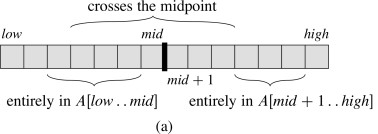
\includegraphics[scale=2.5]{img/subarrays-casos.jpg}
    
    Como i < j, i no puede estar en [(n/2) + 1 .. n] si j esta en el otro rango. 
    
\end{frame}

\begin{frame}
    Lo recién planteado nos acerca aún más al merge sort, ya que podemos resolver dividir el arreglo
    en dos mitades, y resolver recursivamente en cada una de ellas. Esto nos daría i, j en el primer y segundo caso.
    
    
    ¿Y los del tercero?
    
    
\end{frame}



\end{document}
